%%%%%%%%%%%%
%%%%%%%%%%%%
\begin{figure}
\centering
%%%%%%%%%%%%
\pgfdeclarelayer{background}
\pgfsetlayers{background,main}
%%%%%%%%%%%%
%%%%%%%%%%%%

\begin{subfigure}[t]{.3\textwidth}
	\centering
	\fbox{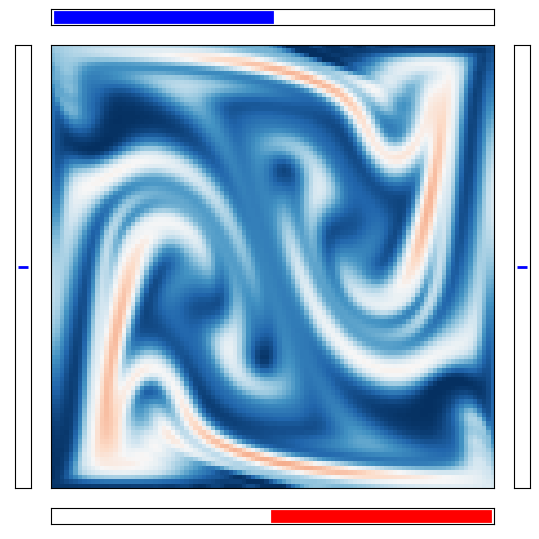
\includegraphics[width=\textwidth]{fig/burgers/t20.png}}
    	\caption{$t=20$}
	\label{fig:burgers_field_20}
\end{subfigure} \quad
\begin{subfigure}[t]{.3\textwidth}
	\centering
	\fbox{\includegraphics[width=\textwidth]{fig/burgers/t40.png}}
    	\caption{$t=40$}
	\label{fig:burgers_field_40}
\end{subfigure} \quad
\begin{subfigure}[t]{.3\textwidth}
	\centering
	\fbox{\includegraphics[width=\textwidth]{fig/burgers/t60.png}}
    	\caption{$t=60$}
	\label{fig:burgers_field_60}
\end{subfigure}

\medskip

\begin{subfigure}[t]{.3\textwidth}
	\centering
	\fbox{\includegraphics[width=\textwidth]{fig/burgers/t100.png}}
    	\caption{$t=100$}
	\label{fig:burgers_field_100}
\end{subfigure} \quad
\begin{subfigure}[t]{.3\textwidth}
	\centering
	\fbox{\includegraphics[width=\textwidth]{fig/burgers/t150.png}}
    	\caption{$t=150$}
	\label{fig:burgers_field_150}
\end{subfigure} \quad
\begin{subfigure}[t]{.3\textwidth}
	\centering
	\fbox{\includegraphics[width=\textwidth]{fig/burgers/t200.png}}
    	\caption{$t=200$}
	\label{fig:burgers_field_200}
\end{subfigure}

%%%%%%%%%%%%
\caption{\textbf{Evolution of the controlled burgers system} using the \ppo algorithm. The instantaneous control value is indicated at the bottom by the colored bar (blue is for negative actuations, while red is for positive ones).}
\label{fig:burgers_fields}
\end{figure} 
%%%%%%%%%%%%
%%%%%%%%%%%%